\documentclass[11pt]{article}
\usepackage[a4paper, margin=0.5in]{geometry}
\usepackage{cite}
\usepackage{amsmath,amssymb,amsfonts}
\usepackage{algorithmic}
\usepackage[export]{adjustbox}
\usepackage{graphicx}
\usepackage{textcomp}
\usepackage{listings}
\usepackage{matlab-prettifier}
\usepackage{tabularx}
\usepackage{caption}
\usepackage{subcaption}
\usepackage{url}
\usepackage{hyperref}
\usepackage{array}
\usepackage{lastpage}
\raggedbottom
\usepackage{cite}
\usepackage{indentfirst}
\usepackage{fancyhdr}
\renewcommand*\contentsname{TABLE OF CONTENTS}
\renewcommand{\listfigurename}{List of Figures}
\begin{document}
\tableofcontents
\listoffigures
\pagestyle{fancy}
\fancyhead{}
\fancyhead[LO,LE]{Name: Md. Raisul Islam Rifat}
\fancyhead[RO,RE]{ID: 1902081}
\fancyfoot{}
\fancyfoot[RE,RO]{Page \thepage\ of \pageref{LastPage}}
\newpage
\section{Abstract}
This document outlines the design and simulation of a 2-input NAND gate 
using Cadence Virtuoso. The design process involves creating a schematic, 
symbol, and performing the necessary simulations to verify the 
functionality of the NAND gate. Initially, the transistor-level schematic is 
designed using PMOS and NMOS transistors configured in a 
complementary arrangement. Following the schematic creation, a symbol 
view is generated for hierarchical design use. The layout design involves 
placing and routing the transistors, ensuring proper connectivity and 
adherence to design rules. Check and save process is conducted to ensure 
correctness. Finally, simulations, including DC, transient, and parametric 
analyses, are performed to verify the gate's logical functionality and 
performance metrics.
\section{Keywords}
2-input NAND Gate, Rise time, Fall time, Propagation delay
\section{Objectives}
\begin{enumerate}
\item To login in to the Cadence Server shell and start the Cadence virtuoso
software
\item To create a working library
\item To draw the schematic of a 2-input NAND gate in Cadence Virtuoso
Schematic Editor
\item To create a symbol view of the NAND gate from the schematic
\item To simulate the NAND gate using MMSIM Spectre
\item To determine the rise time and fall time of the output waveforms.
\end{enumerate}
\section{Introduction}
By performing this experiment, we will learn about the usage of 
CADENCE VIRTUOSO. We will also learn about the addition process 
of the libraries (basic, analogLib, gpdk090). We will also learn about the 
making process about the schematic, symbol and simulate, outputting 
the signals. We will also learn about the propagation delay, rise time, 
fall time.
\section{Theory}
NAND gate is a fundamental digital logic gate used extensively in digital 
circuits due to its versatility and functional completeness. A NAND gate 
performs the logical NAND operation, where the output is true (or high) 
unless both inputs are true (or high). This gate is a building block for 
various digital systems, including arithmetic logic units, memory storage, 
and more complex logic circuits. Designing a 2-input NAND gate in Cadence Virtuoso, an advanced electronic design automation (EDA) tool, 
involves a series of methodical steps, from schematic capture to simulation.
Cadence Virtuoso offers a comprehensive environment for the design and 
verification of custom ICs, providing tools for schematic entry, layout 
editing, and extensive simulation capabilities. The process begins with 
creating a transistor-level schematic of the NAND gate using PMOS and 
NMOS transistors. This is followed by generating a symbol for the NAND 
gate, enabling its use in hierarchical design contexts. The next step is the 
simulation.
\newpage
\section{Truth Table}
\begin{center}
\begin{tabular}{|c|c|c|c|c|}
\hline 
\hline
A (input) & B (input) & Pull Down Network & Pull Up Network & O (output) \\ 
\hline 
\hline
0 & 0 & Off & On & 1 \\ 
\hline 
0 & 1 & Off & On & 1 \\ 
\hline 
1 & 0 & Off & On & 1 \\ 
\hline 
1 & 1 & On & Off & 0 \\ 
\hline 
\end{tabular}
\end{center}
\section{Propagation Delay}
\subsection{$\text{P}_{mos}=240\text{ }nm$, $\text{N}_{mos}=240\text{ }nm$ }
\begin{center}
\begin{tabular}{|c|c|c|}
\hline 
A (input) & O (output) & Propagation Delay $(s)$ \\ 
\hline 
falling & falling & $5.006\times10^{-9}$ \\ 
\hline 
falling & rising & $8.201\times10^{-12}$ \\ 
\hline 
rising & falling & $6.254\times10^{-12}$ \\ 
\hline 
rising & rising & $4.992\times10^{-12}$ \\ 
\hline 
\end{tabular} 
\end{center}
\subsection{$\text{P}_{mos}=240\text{ }nm$, $\text{N}_{mos}=120\text{ }nm$ }
\begin{center}
\begin{tabular}{|c|c|c|}
\hline 
A (input) & O (output) & Propagation Delay $(s)$ \\ 
\hline 
falling & falling & $5.01\times10^{-9}$ \\ 
\hline 
falling & rising & $7.228\times10^{-12}$ \\ 
\hline 
rising & falling & $9.79\times10^{-12}$ \\ 
\hline 
rising & rising & $4.993\times10^{-12}$ \\ 
\hline 
\end{tabular} 
\end{center}
\section{Simulation Setup}
\begin{figure}[!h]
\begin{subfigure}[h]{0.5\textwidth}
\centering
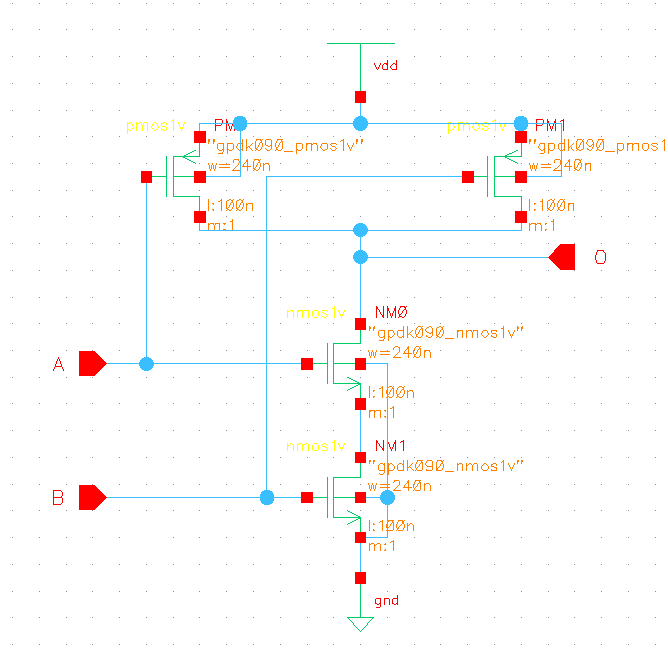
\includegraphics[width=\linewidth]{sch240}
\caption{Schematic where $\text{P}_{mos}=240\text{ }nm$, $\text{N}_{mos}=240\text{ }nm$ }
\label{fig:sub-a}
\end{subfigure}
\begin{subfigure}[h]{0.5\textwidth}
\centering
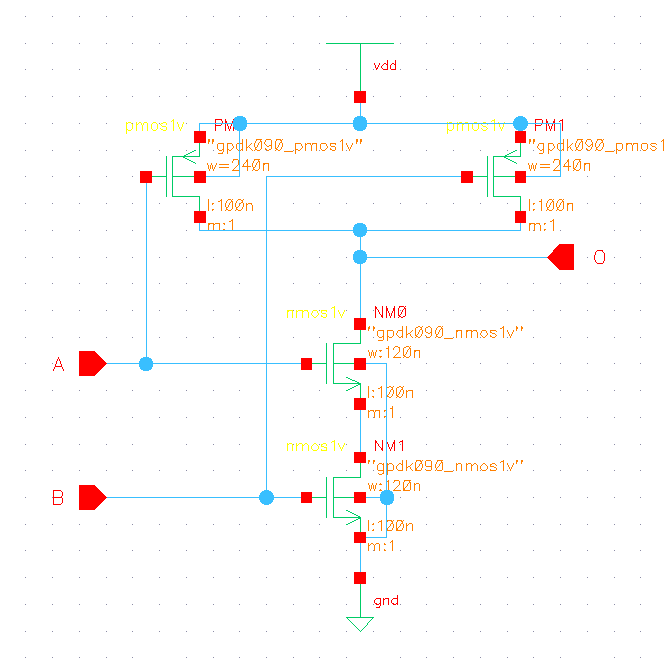
\includegraphics[width=\linewidth]{sch120}
\caption{Schematic where $\text{P}_{mos}=240\text{ }nm$, $\text{N}_{mos}=120\text{ }nm$ }
\label{fig:sub-b}
\end{subfigure}
\caption{Internal circuitry of NAND gates}
\end{figure}
\newpage
\begin{figure}[!h]
\begin{subfigure}[h]{\textwidth}
\centering
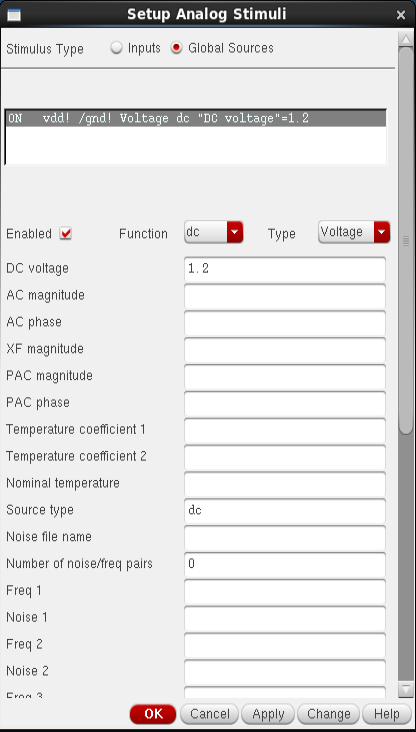
\includegraphics[width=0.475\textwidth, height=0.45\textheight]{globalparams}
\caption{Parameter selection for global source}
\end{subfigure}
\begin{subfigure}[h]{0.5\textwidth}
\centering
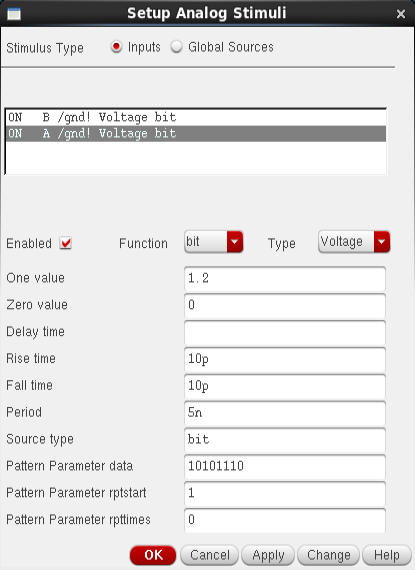
\includegraphics[width=0.95\textwidth, height=0.45\textheight]{Aparams}
\caption{Parameter selection for input A}
\end{subfigure}
\begin{subfigure}[h]{0.5\textwidth}
\centering
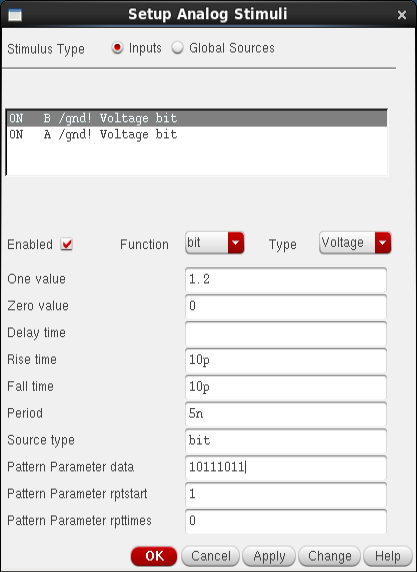
\includegraphics[width=0.95\textwidth, height=0.45\textheight]{Bparams}
\caption{Parameter selection for input B}
\end{subfigure}
\caption{Definition of Input Parameters}
\end{figure}
\newpage
\section{Simulation Result}
\begin{figure}[!h]
\centering
\begin{subfigure}[h]{\textwidth}
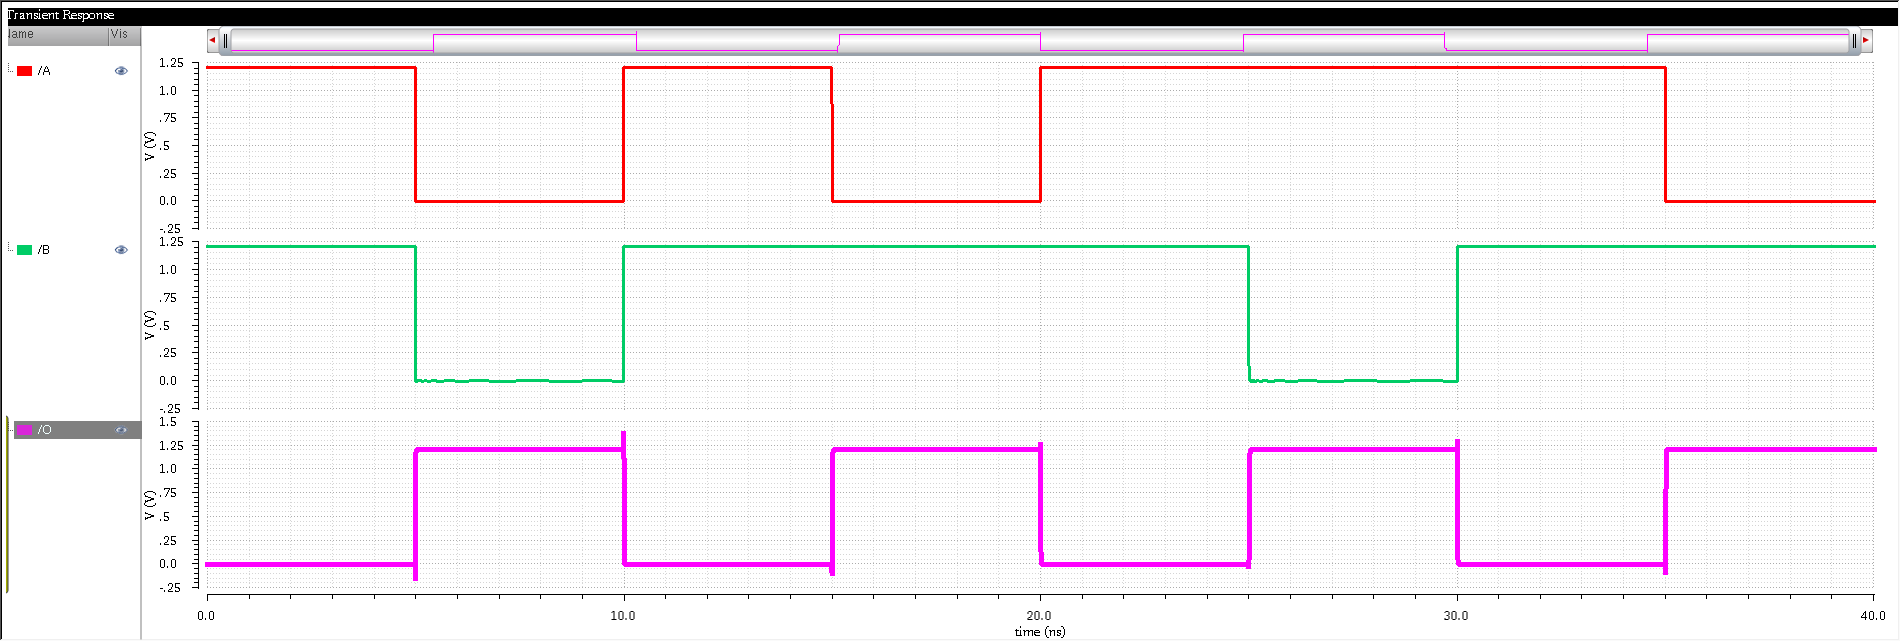
\includegraphics[width=\textwidth,height=0.43\textheight]{sym240}
\caption{Output wave forms for $\text{P}_{mos}=240\text{ }nm$, $\text{N}_{mos}=240\text{ }nm$}
\end{subfigure}
\begin{subfigure}[h]{\textwidth}
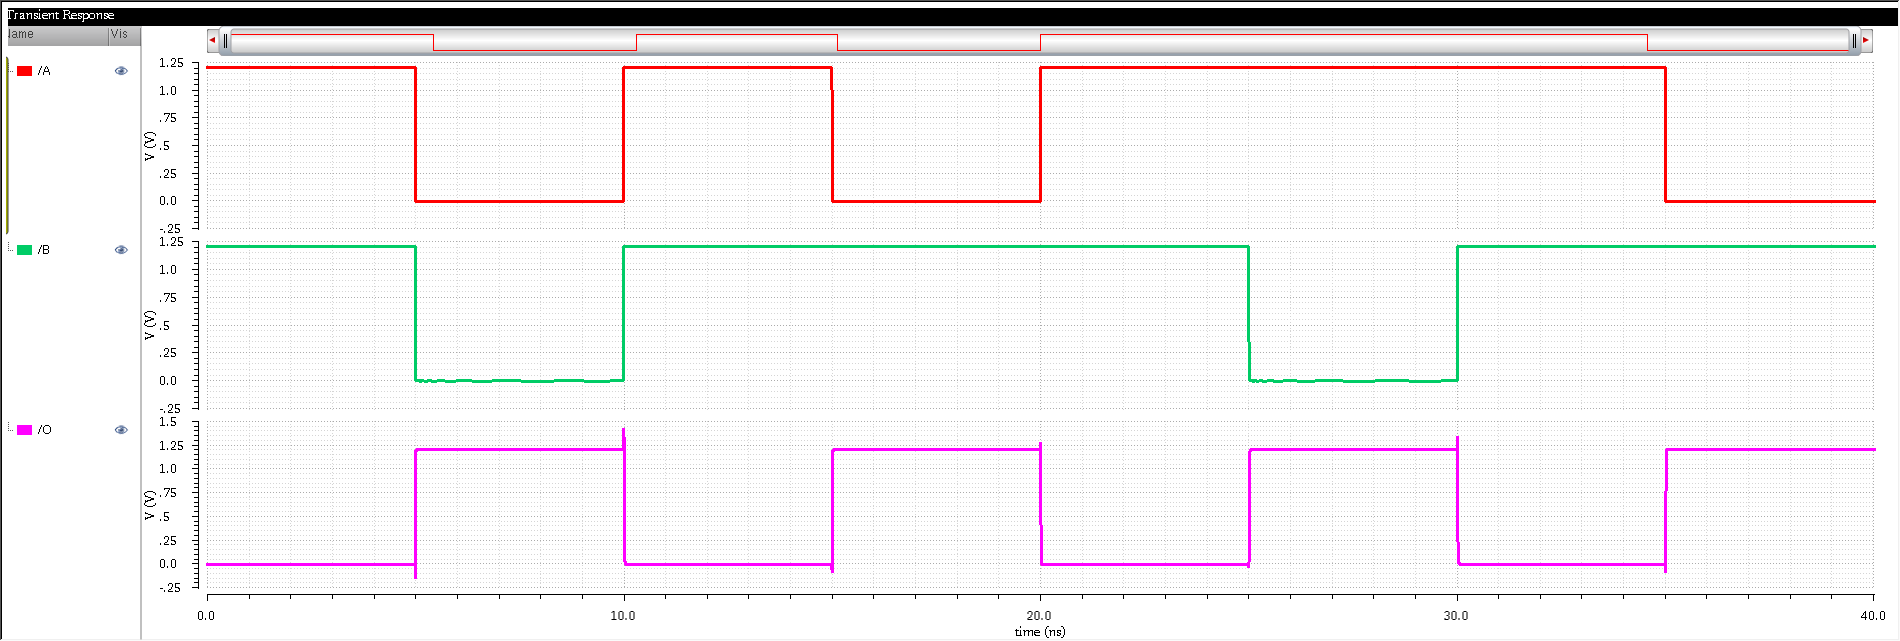
\includegraphics[width=\textwidth,height=0.43\textheight]{sym120}
\caption{Output wave forms for $\text{P}_{mos}=240\text{ }nm$, $\text{N}_{mos}=120\text{ }nm$}
\end{subfigure}
\caption{Input and Output waveforms of NAND Gates}
\end{figure}
\newpage
\begin{figure}[!h]
\centering
\begin{subfigure}[h]{\textwidth}
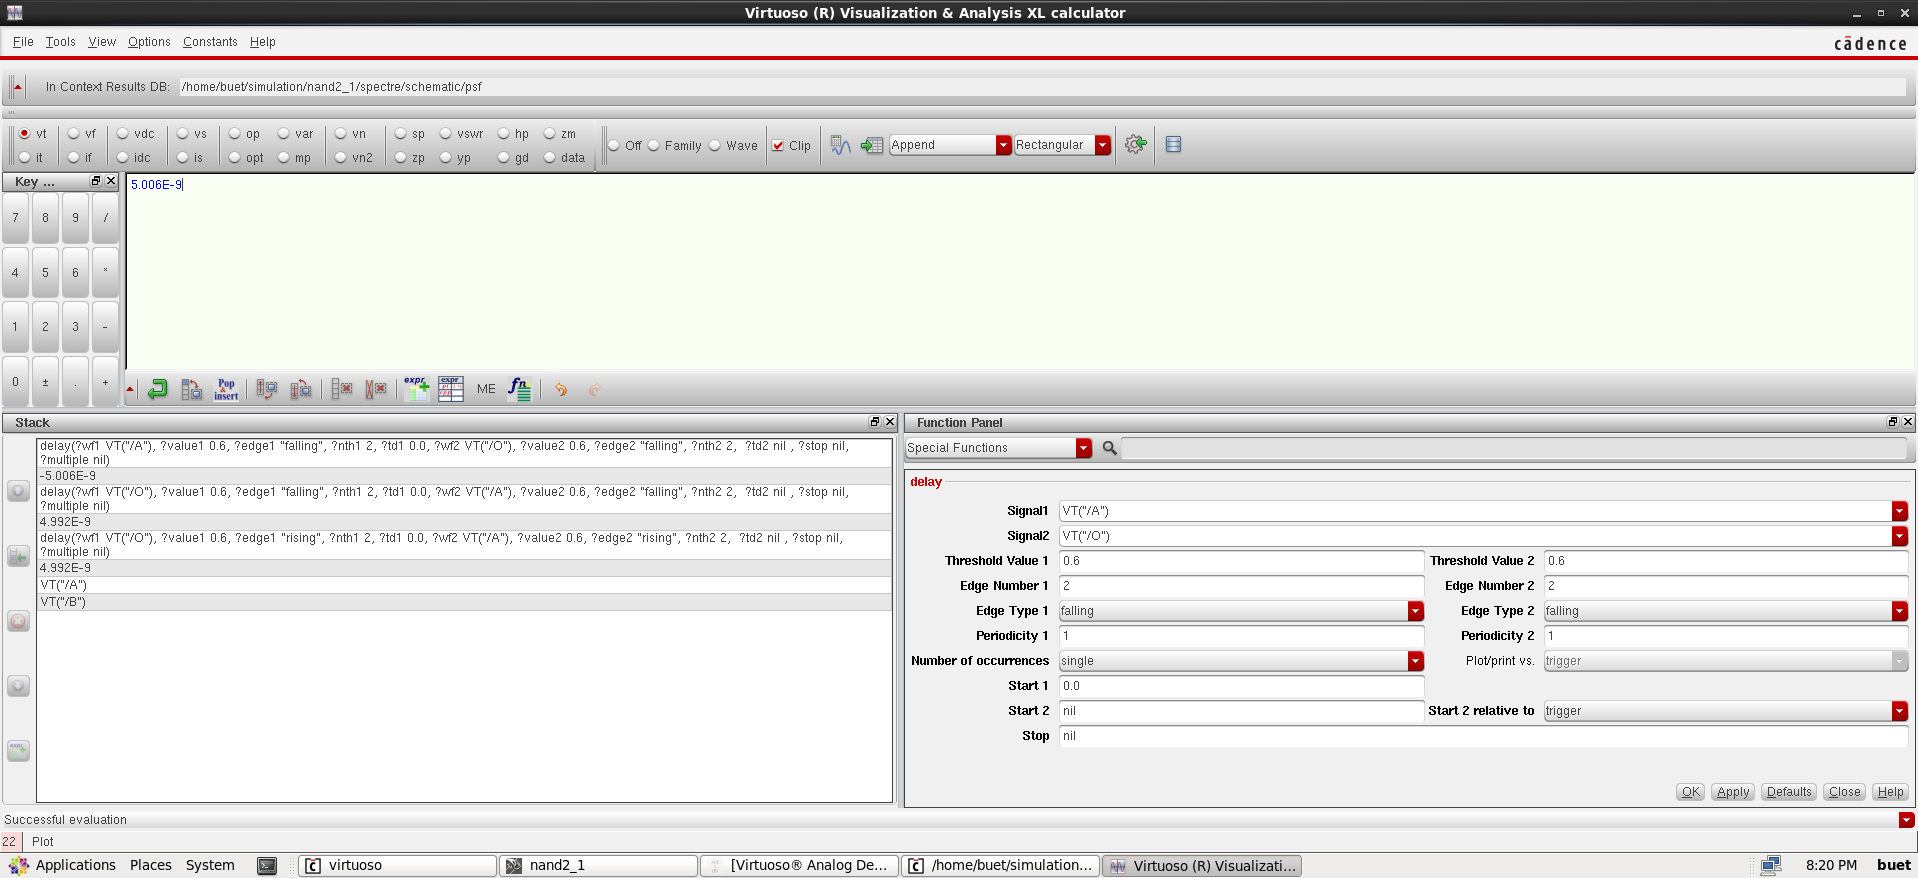
\includegraphics[width=\textwidth,height=0.43\textheight]{00240}
\caption{When both edges are falling}
\end{subfigure}
\begin{subfigure}[h]{\textwidth}
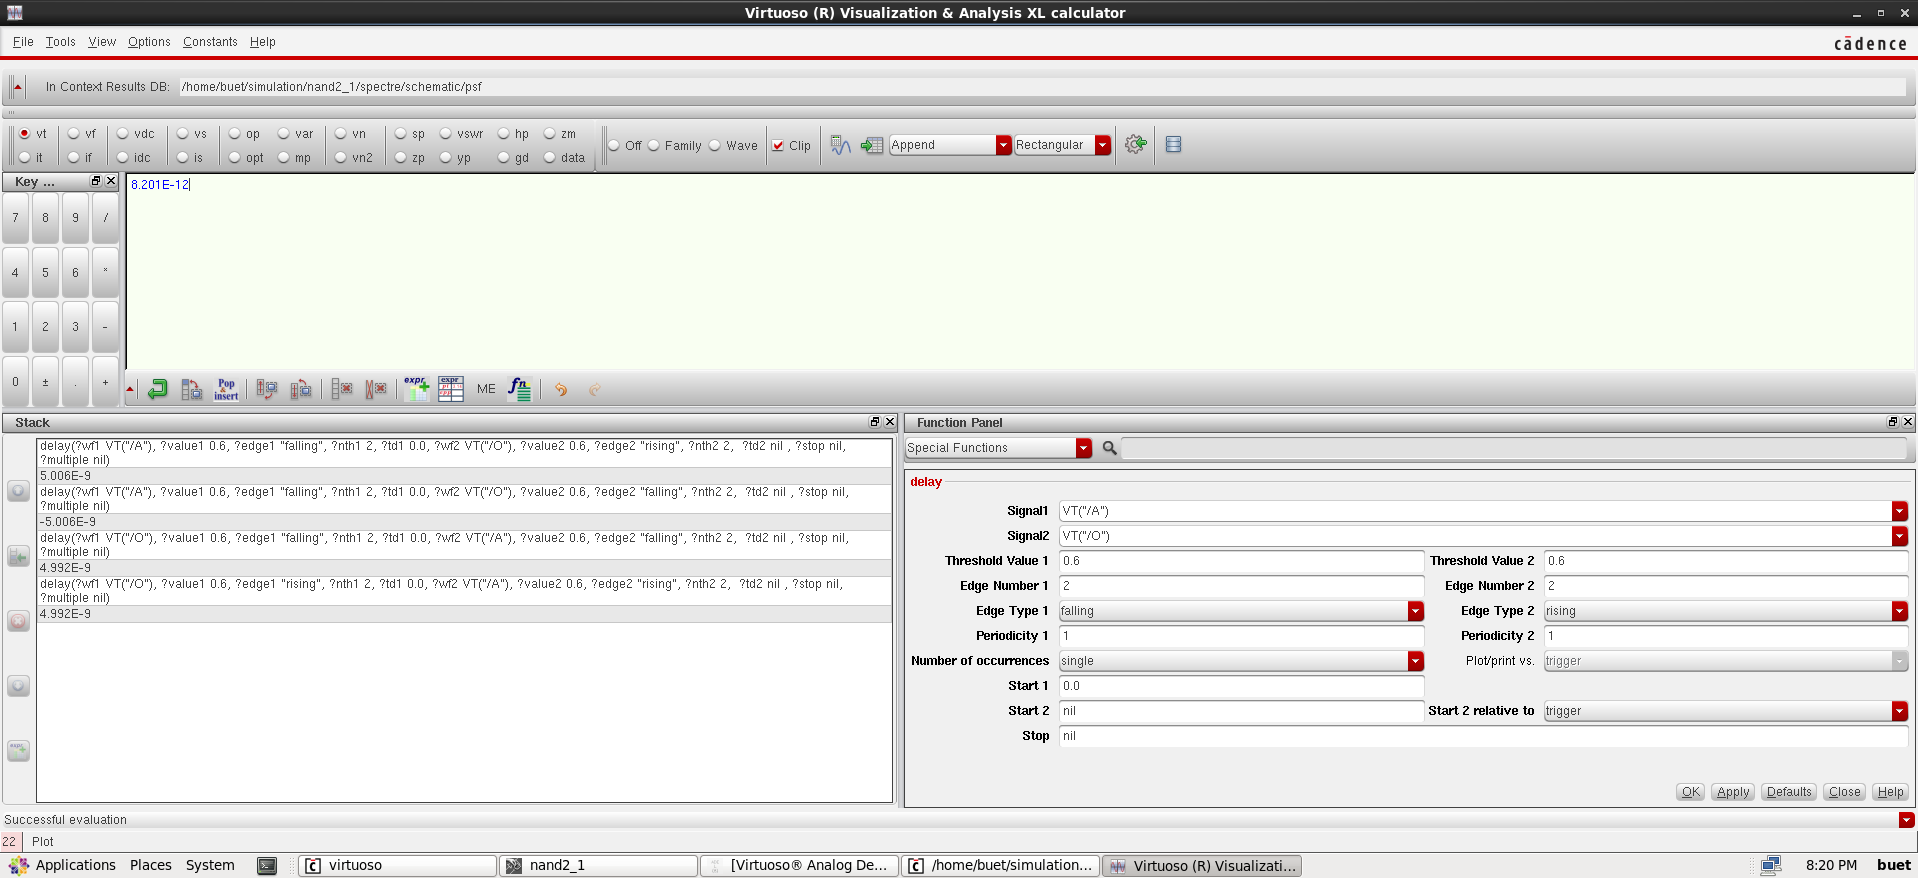
\includegraphics[width=\textwidth,height=0.43\textheight]{01240}
\caption{When edge 1 is falling but edge 2 is rising}
\end{subfigure}
\end{figure}
\newpage
\begin{figure}[!h]
\continuedfloat
\centering
\begin{subfigure}[h]{\textwidth}
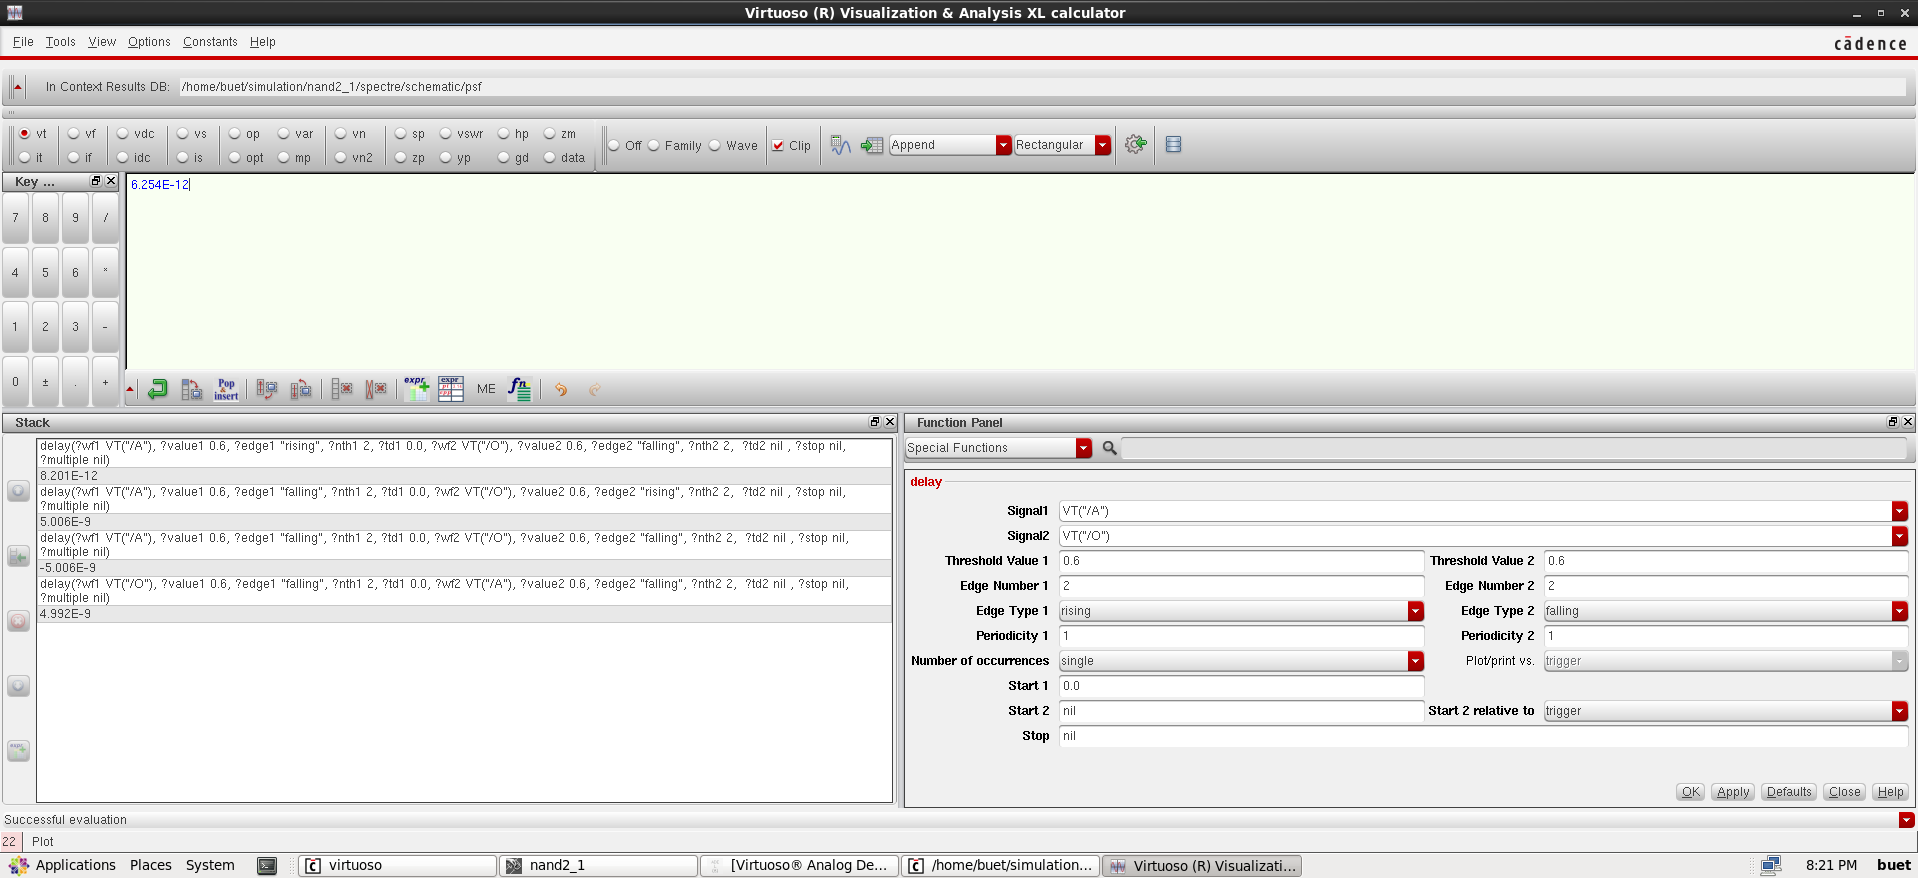
\includegraphics[width=\textwidth,height=0.43\textheight]{10240}
\caption{When edge 1 is rising but edge 2 is falling}
\end{subfigure}
\begin{subfigure}[h]{\textwidth}
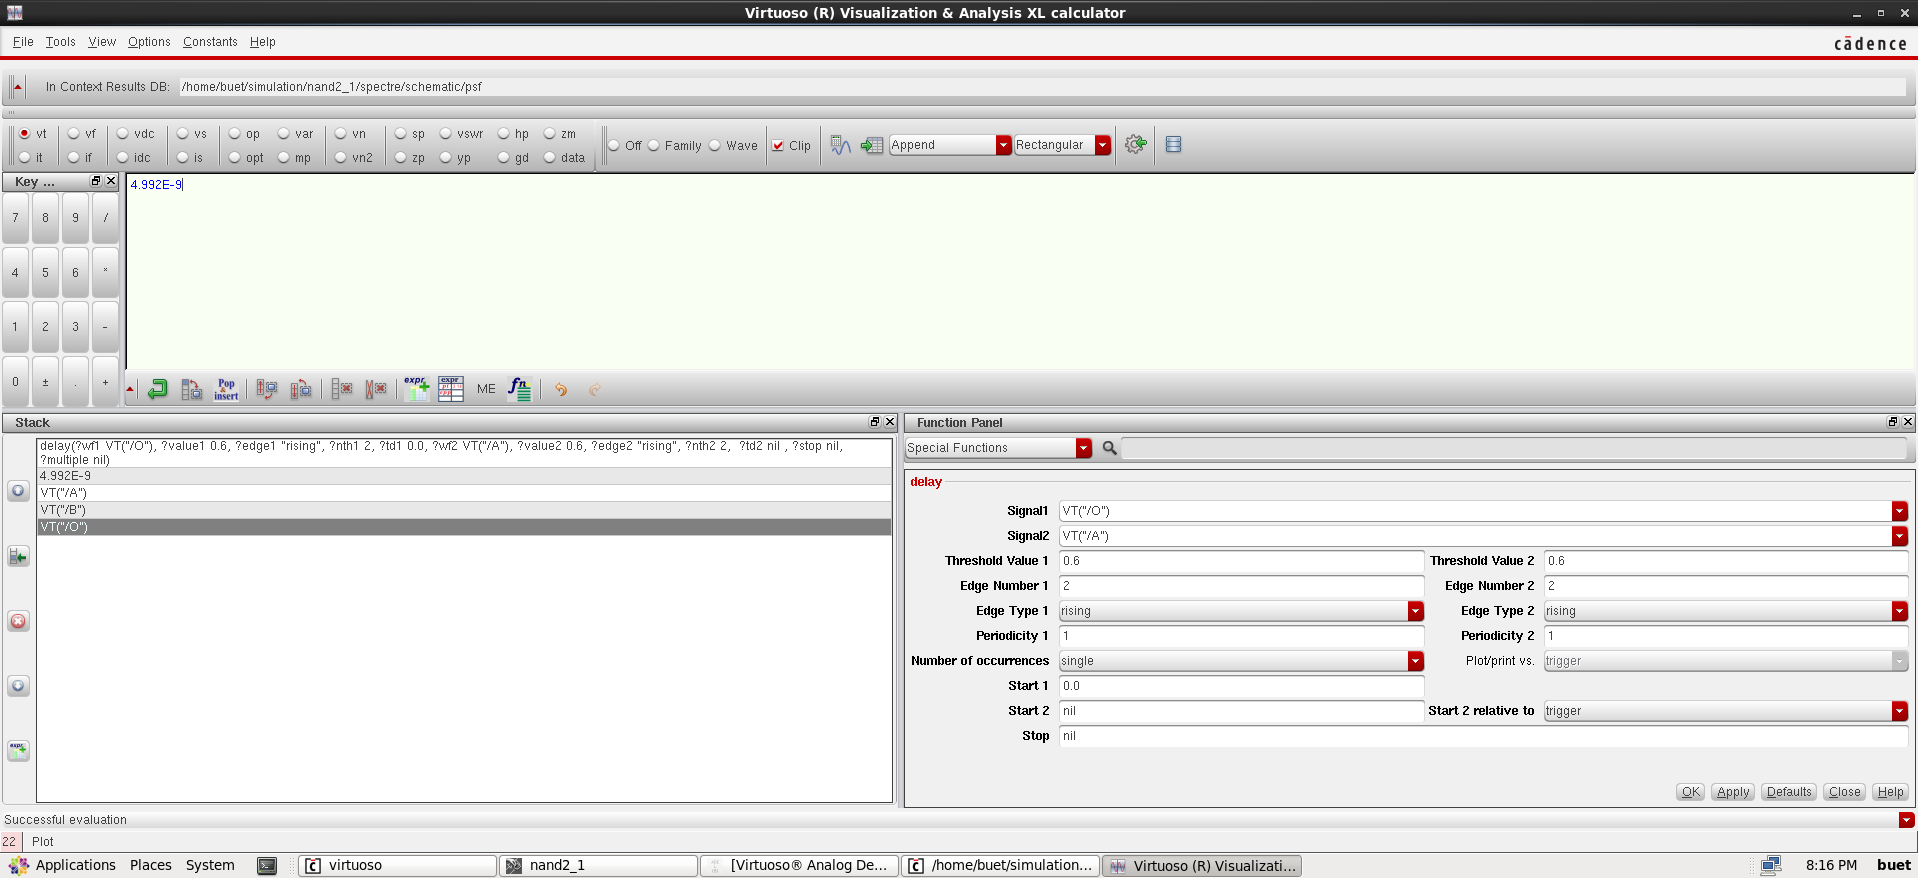
\includegraphics[width=\textwidth,height=0.43\textheight]{11240}
\caption{When both edges are rising}
\end{subfigure}
\caption{Propagation delay for $240\text{ }nm$ $\text{N}_{mos}$ architecture}
\end{figure}
\newpage
\begin{figure}[!h]
\centering
\begin{subfigure}[h]{\textwidth}
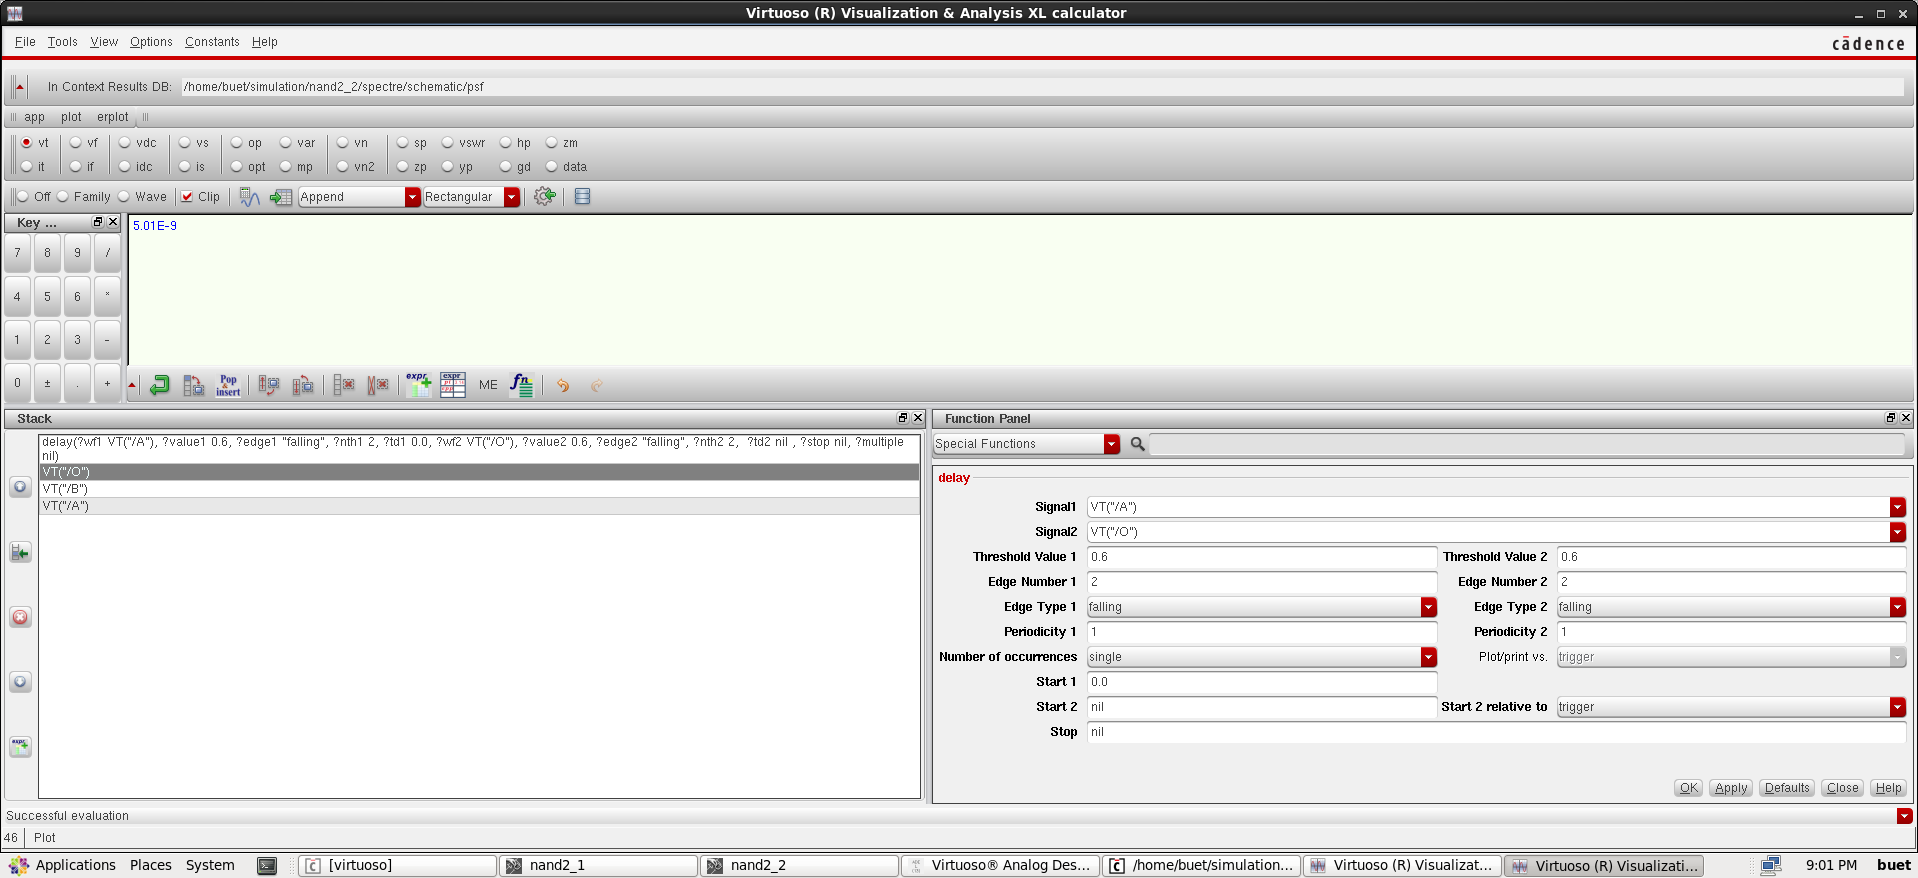
\includegraphics[width=\textwidth,height=0.43\textheight]{00120}
\caption{When both edges are falling}
\end{subfigure}
\begin{subfigure}[h]{\textwidth}
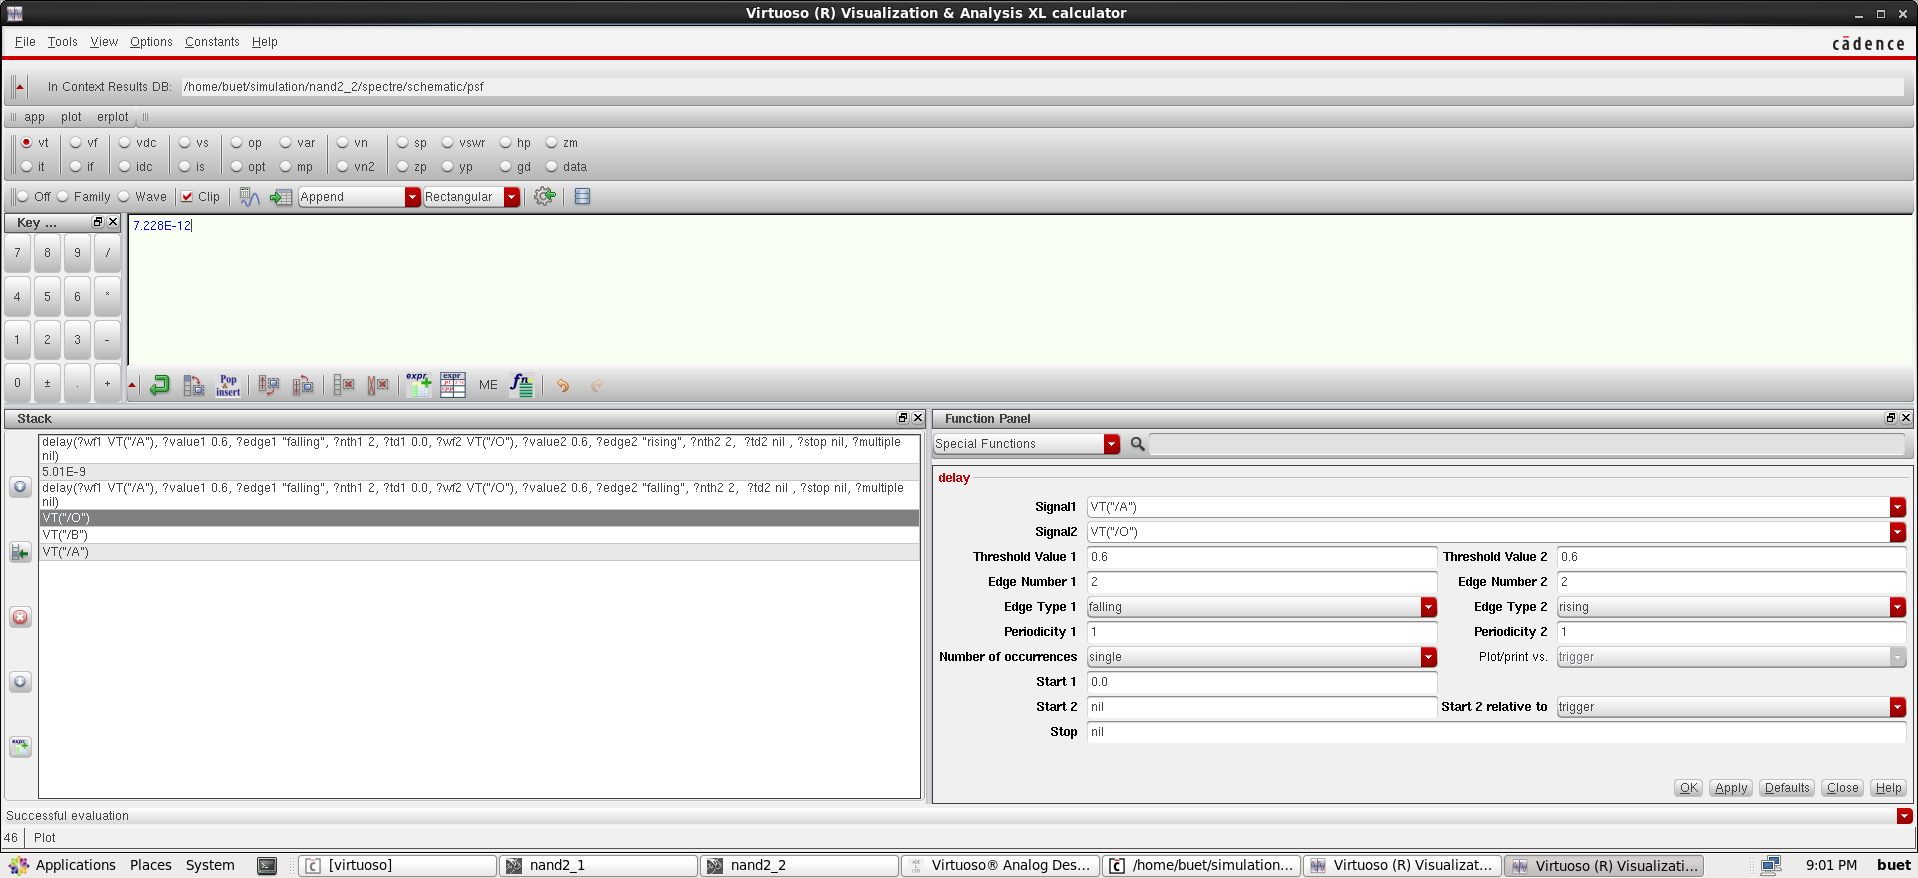
\includegraphics[width=\textwidth,height=0.43\textheight]{01120}
\caption{When edge 1 is falling but edge 2 is rising}
\end{subfigure}
\end{figure}
\newpage
\begin{figure}[!h]
\continuedfloat
\centering
\begin{subfigure}[h]{\textwidth}
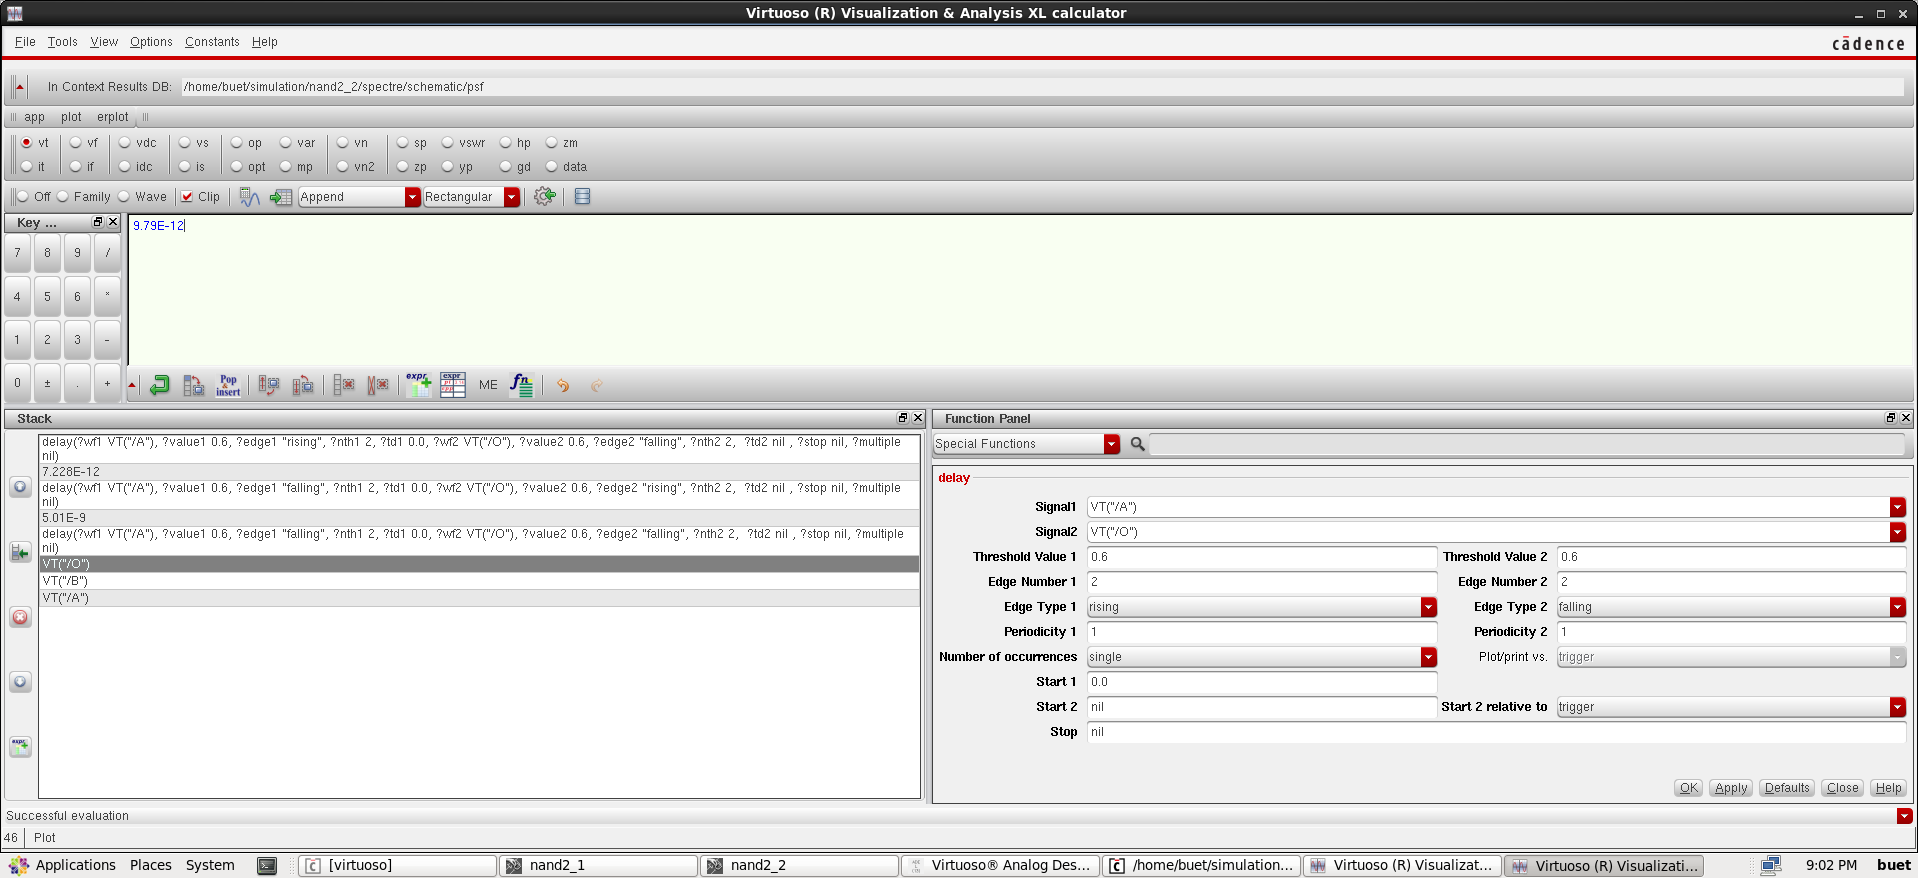
\includegraphics[width=\textwidth,height=0.43\textheight]{10120}
\caption{When edge 1 is rising but edge 2 is falling}
\end{subfigure}
\begin{subfigure}[h]{\textwidth}
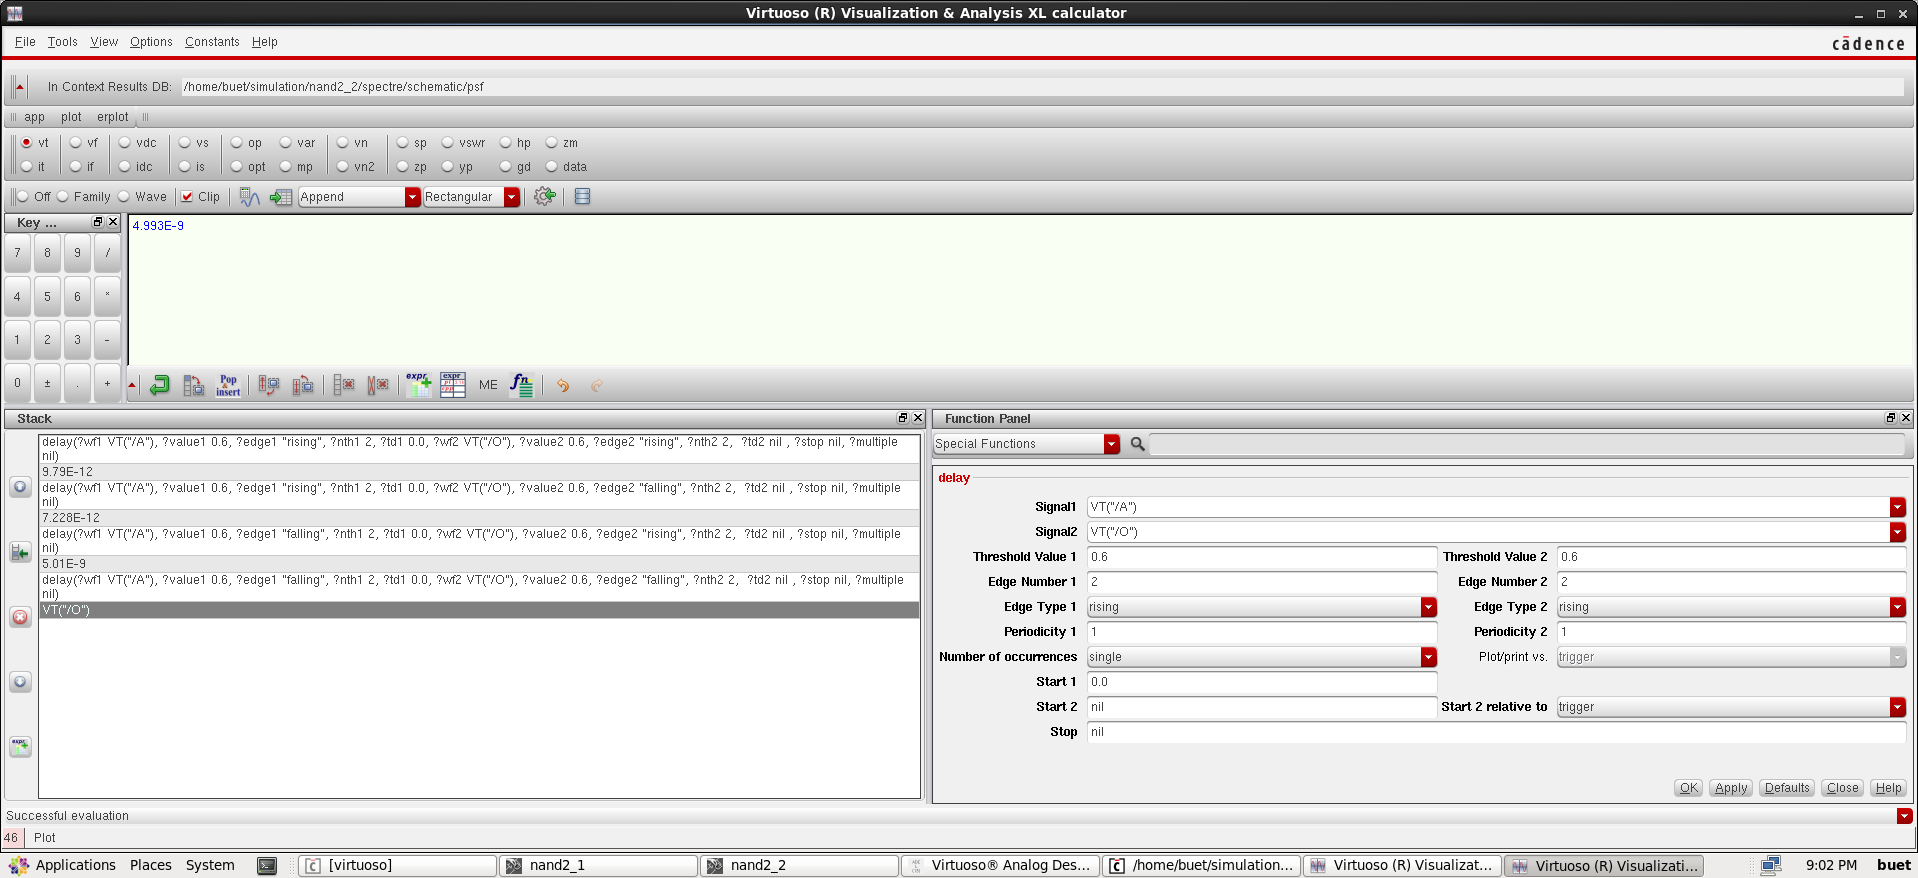
\includegraphics[width=\textwidth,height=0.43\textheight]{11120}
\caption{When both edges are rising}
\end{subfigure}
\caption{Propagation delay for $120\text{ }nm$ $\text{N}_{mos}$ architecture}
\end{figure}
\newpage
\section{Tools Used}
\begin{enumerate}
\item Cadence Virtuoso.
\item VMware Hypervisor.
\end{enumerate}
\section{Conclusion}
In this experiment, we became acquainted with Cadence Software. We 
created the schematic for a 2-input NAND gate and identified the required 
parameters and waveforms. We also prepared a truth table and compared 
it with the simulation results.
\section{References}
\begin{enumerate}
\item Lab Manual.
\item Cadence Virtuoso Tutorial - University of Southern California.
\end{enumerate}
\end{document}